\chapter{Background}

\section{Sicurezza Industriale e DPI}

La sicurezza sul lavoro nell'industria manifatturiera è di primaria importanza per garantire non solo la salute e il benessere dei lavoratori, ma anche l'efficienza operativa e la sostenibilità economica delle aziende. Secondo i dati forniti dall'Istituto Nazionale per l'Assicurazione contro gli Infortuni sul Lavoro (INAIL), nel 2022 il settore manifatturiero ha registrato un tasso di infortuni del 13,9\% sul totale \cite{inail2023}.

\begin{figure}[htbp]
    \centering
    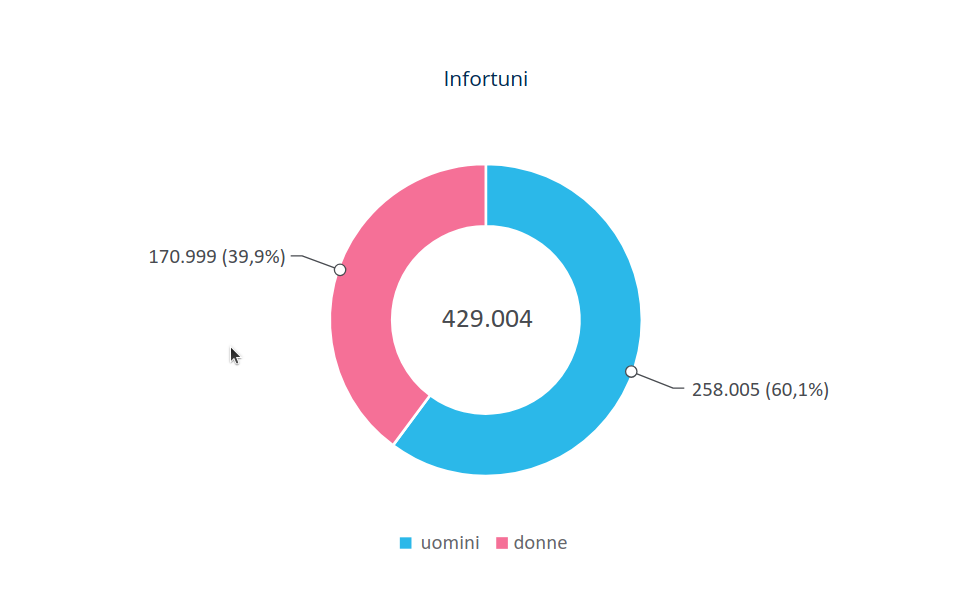
\includegraphics[width=0.8\textwidth]{figures/totaleinfortuni.png}
    \caption{Infortuni sul lavoro accertati positivi per genere
e modalità di accadimento nell'anno 2022.}
    \label{fig:infortot}
\end{figure}

\begin{figure}[htbp]
    \centering
    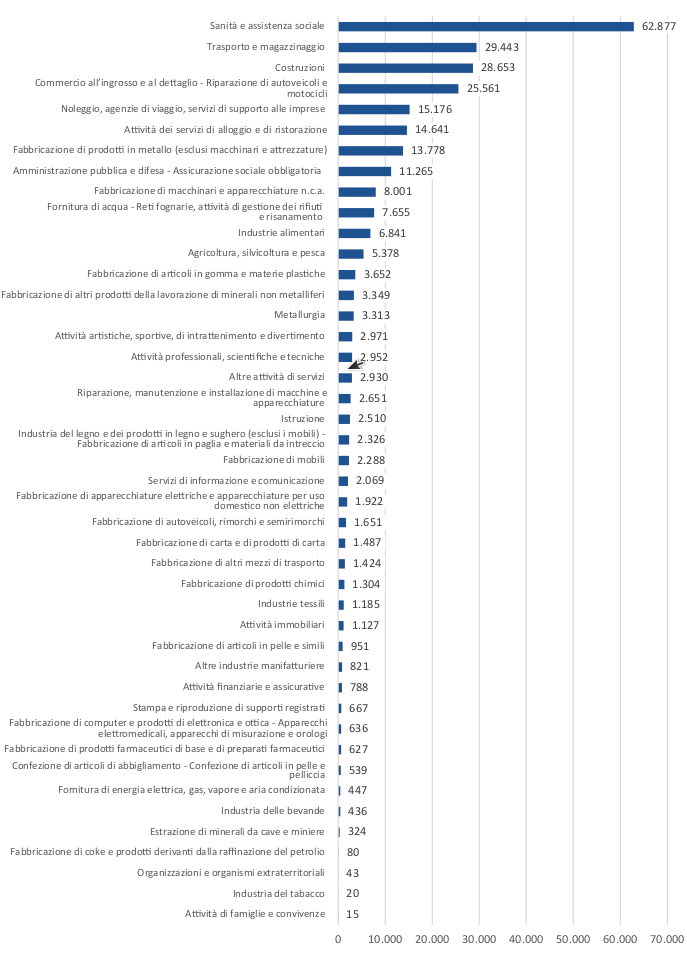
\includegraphics[width=0.8\textwidth]{figures/infortuni_industria_e_servizi.png}
    \caption{infortuni in occasione di lavoro accertati positivi per settore di attività nell'anno 2022}
    \label{fig:infortot}
\end{figure}

Essi comportano gravi conseguenze per i dipendenti, inclusi infortuni permanenti, invalidità e, nei casi più gravi, decessi. Oltre al costo umano, gli incidenti sul lavoro hanno un impatto significativo sull'economia delle aziende, generando costi diretti come spese mediche e indennità di infortunio, e costi indiretti come perdita di produttività, danni reputazionali e aumento dei premi assicurativi. L'EU-Occupational Safety and Health Administration (EU-OSHA) a questo proposito ha stimato in due diversi approcci l'impatto degli incidenti sul lavoro all'interno dell'Unione Europea\cite{osha-eu}. Nell'indagine sono stati presi in esame i dati relativi a 5 Paesi, poiché più completi e accessibili, tra cui figura anche l'Italia e sono stati mostrati i risultati seguendo due diversi approcci: uno bottom-up, perché prende i valori dei costi per ciascun infortunio e li valuta globalmente; l'altro top-down, in quanto stima stima l'impatto dell'infortunio sulla vita del lavoratore e da valori macroeconomici come il PIL pro-capite valuta il costo effettivo dell'infortunio sul singolo. In termini pratici, nel primo caso si tiene conto dei costi diretti, indiretti e immateriali (effetti sulla vita e sulla salute) mentre nel secondo del valore monetario espresso in DALY, cioè il costo in termini di anni di vita persi a causa di un infortunio o di una malattia.

\vspace{0,5cm}
\begin{figure}[htbp]
    \centering
    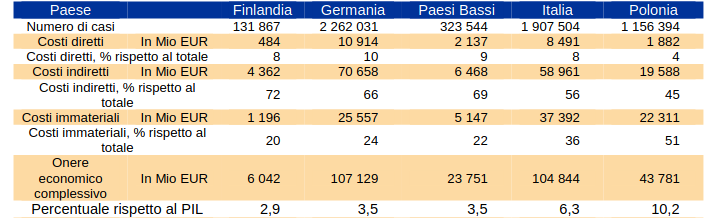
\includegraphics[width=\textwidth]{figures/onere_infortuni_ba.png}
    \caption{onere economico complessivo stimato (approccio bottom up)}
    \label{fig:osha_table1}
\end{figure}
\vspace{0,5cm} 

\noindent Il risultato di queste analisi ha mostrato che per l'Italia il costo di un infortunio o malattia causata dal posto di lavoro aveva un impatto percentuale sul PIL del 6,3\% nel primo caso, mentre nell'approccio top down, riferendosi alla metodologia VSLY - considerata più coerente con i risultati dell'approccio bottom up - il valore medio era del 7,7\% rispetto alla produzione interna. Da questi valori quindi si può dedurre quanto questo problema sia reale e impatti sulla società e sull'economia dell'Italia, dove il posto di lavoro è in gran parte costituito dall'industria. 
 
\begin{figure}[H]
    \centering
    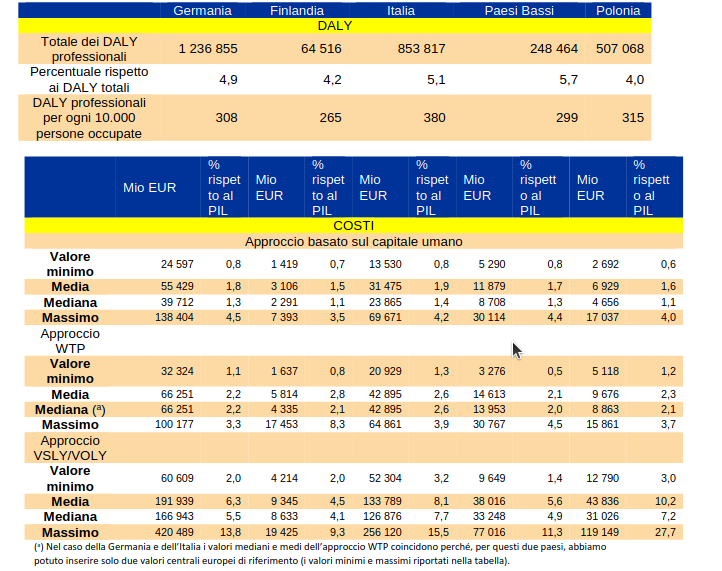
\includegraphics[width=0.8\textwidth]{figures/onere_infortuni_td.png}
    \caption{stima dei costi complessivi approccio top down}
    \label{fig:osha_table2}
\end{figure} 

**********da revisionare***********************************************************
\noindent L'utilizzo corretto dei Dispositivi di Protezione Individuale (DPI) è fondamentale per prevenire tali incidenti. I DPI sono strumenti progettati per proteggere i lavoratori da rischi specifici presenti nell'ambiente di lavoro. Tra i DPI più comuni nell' industria manifatturiera troviamo:

\begin{itemize}
    \item \textbf{Caschi Protettivi}: Proteggono la testa da urti, cadute di oggetti e altre lesioni fisiche. Sono essenziali in ambienti dove operano macchinari pesanti o dove vi è rischio di caduta di materiali.
    \item \textbf{Guanti Protettivi}: Offrono protezione alle mani contro tagli, abrasioni, sostanze chimiche e alte temperature. La scelta del tipo di guanto dipende dal rischio specifico presente nell'ambiente di lavoro.
    \item \textbf{Occhiali Protettivi}: Proteggono gli occhi da particelle volanti, spruzzi di sostanze chimiche e radiazioni nocive. Sono indispensabili in operazioni di taglio, saldatura e manipolazione di materiali pericolosi.
    \item \textbf{Indumenti di Protezione}: Comprendono tute, grembiuli e abbigliamento resistente al fuoco, progettati per proteggere il corpo dai rischi specifici dell'ambiente industriale.
    \item \textbf{Protezioni Uditive}: Come tappi per le orecchie e cuffie antirumore, utilizzate in ambienti con livelli elevati di rumore per prevenire danni all'udito \cite{dpisicurezza}.
    \item \textbf{Mascherine Respiratorie}: Proteggono dalle polveri sottili, vapori e gas nocivi, fondamentali in operazioni di saldatura, verniciatura e manipolazione di sostanze chimiche.
\end{itemize}

L'efficacia dei DPI dipende dall'uso corretto e dalla loro manutenzione regolare. È fondamentale che i lavoratori ricevano una formazione adeguata sull'uso e l'importanza dei DPI, e che le aziende garantiscano la disponibilità di DPI adeguati e in buono stato. Inoltre, i DPI devono essere sostituiti periodicamente e ispezionati per garantirne l’integrità e la funzionalità \cite{dpisicurezza}.

Le normative vigenti in Italia, principalmente il Decreto Legislativo 81/2008, noto come Testo Unico sulla Sicurezza sul Lavoro, regolamentano l'uso dei DPI \cite{decreto81}. Questo decreto stabilisce le disposizioni generali per la tutela della salute e della sicurezza dei lavoratori, specificando le responsabilità dei datori di lavoro nell'analisi dei rischi e nella fornitura di DPI appropriati. Secondo l'articolo 77, i datori di lavoro devono fornire ai lavoratori i DPI necessari per proteggersi dai rischi identificati, garantendo che siano adeguati al tipo di attività svolta e conformi alle normative vigenti.

Il Decreto 81/2008 stabilisce inoltre che i DPI devono essere utilizzati come ultima linea di difesa, dopo aver adottato misure di prevenzione e protezione collettive. Questo principio di gerarchia delle misure di prevenzione sottolinea l'importanza di eliminare o ridurre i rischi a monte prima di affidarsi ai DPI. Inoltre, il decreto prevede che i DPI siano forniti gratuitamente ai lavoratori, che devono essere informati e formati sull'uso corretto degli stessi, e che venga effettuata una valutazione periodica della loro efficacia e conformità \cite{decreto81}.

Le aziende hanno l'obbligo legale di garantire la sicurezza e la salute dei propri dipendenti, conformemente alle leggi nazionali e alle direttive europee. Questo obbligo non è solo un dovere giuridico, ma anche un imperativo morale che riflette l'etica aziendale e il rispetto per la dignità umana. La mancata osservanza delle normative sulla sicurezza può comportare gravi conseguenze legali, incluse sanzioni economiche e responsabilità penali in caso di incidenti gravi \cite{decreto81}.

Sul piano morale, le aziende hanno la responsabilità di proteggere i propri lavoratori non solo per adempiere agli obblighi legali, ma anche per promuovere un ambiente di lavoro sano e sicuro che favorisca il benessere e la produttività. Un impegno serio nella sicurezza sul lavoro contribuisce a costruire una cultura aziendale positiva, migliorando la motivazione e la fidelizzazione dei dipendenti, e rafforzando la reputazione dell'azienda sul mercato \cite{valoresicurezza}.

In conclusione, la sicurezza industriale e l'uso corretto dei DPI sono elementi fondamentali per prevenire gli incidenti sul lavoro e proteggere la salute dei lavoratori nell' industria manifatturiera. Le aziende devono adottare un approccio proattivo nella gestione della sicurezza, combinando misure di prevenzione collettive con l'uso appropriato dei DPI, e rispettando rigorosamente le normative vigenti. Solo attraverso un impegno costante e un'attenzione continua alla sicurezza si può garantire un ambiente di lavoro sicuro ed efficiente, a beneficio sia dei lavoratori che delle aziende stesse.


\section{Computer Vision e Sicurezza sul Lavoro}

/***Si introdurrà il concetto di computer vision, spiegando come questa tecnologia permetta alle macchine di interpretare e comprendere le immagini.***/

\noindent La computer vision è una branca del machine learning che ha come scopo l'elaborazione di immagini o di video. I task che si possono svolgere sono di diversi tipi, tra cui spiccano la classificazione, l'object detection, la segmentazione, il riconoscimento di volti, l'encoding, l'applicazione di filtri per la modifica delle immagini originali.

La ricerca nella visione artificiale è stata la prima a mostrare le potenzialità delle reti neurali nei problemi di tutti i giorni. Storicamente è stato l'insieme di diversi sviluppi in discipline differenti ad aver permesso di raggiungere questo traguardo, come la neuroscienza, la modellazione del neurone artificiale e la successiva estensione a più strati, l'utilizzo del calcolo differenziale per l'aggiornamento dei pesi, l'introduzione di funzioni di attivazione e di costo sempre più complesse, che si adattessero meglio al problema da risolvere ed infine la formulazione del teorema di approssimazione universale (r:migliorabile). 

Alla fine degli anni '50 è stato modellato il primo neurone artificiale, ispirandosi al neurone biologico (non valido in generale per la teoria delle reti neurali), composto dalla combinazione lineare di input e pesi in ingresso ad una funzione di attivazione. Questo meccanismo semplice era in grado di mimare grossolanamente la risposta a dei dati in ingresso, in modo tale che, superata una certa soglia, producesse o meno un valore in uscita. La funzione di attivazione era una funzione gradino (al tempo non era scontato generare funzioni non lineari e continue), ma comunque questo oggetto era in grado di risolvere problemi di classificazione. Il limite principale consisteva nell'aggiornamento dei pesi in caso di predizioni sbagliate, basato su una semplice delta di valori discreti. La funzione di aggiornamento dei pesi forniva in maniera euristica una direzione verso l'insieme ottimale delle variabili interne al modello, per ottenere la predizione il più possibile corretta ad ogni nuovo input. 

Per risolvere questi limiti, venne definita una funzione di attivazione continua, trasformando il problema da uno di classificazione ad uno di regressione. Questa nuova costruzione permetteva l'introduzione di una funzione di costo (r: è questa la vera novità, l'aggiornamento non si basava sull'output ma sull'errore, la teoria sulla discesa del gradiente viene adottata solo negli anni 80, nonostante la matematica relativa fosse già stata inventata un secolo prima --> questa parte da aggiustare) che fosse derivabile, potendo così sfruttare il concetto di discesa del gradiente. Effettuando un'operazione di derivazione, si poteva trovare il suo minimo, che in termini pratici significava ridurre il più possibile l'errore nella rappresentazione della funzione che si voleva apprendere dai dati. Fino alla fine degli anni '60 si sperimentò l'utilizzo di questi modelli, di cui gli esempi più famosi sono Adaline e Madaline, costituiti da semplici reti di neuroni artificiali, rispettivamente ad uno e due strati. 

Queste reti non riuscivano a rappresentare correttamente le non linearità presenti nella distribuzione dei dati, ma questo al tempo era solo un limite tecnico e non teorico, poiché non erano ancora state introdotte funzioni di attivazione non lineari continue come la sigmoide e non era ancora stato compreso come propagare l'aggiornamento dei pesi negli strati nascosti. Questo punto è fondamentale nella risoluzione di problemi più complessi, perché solo grazie alla stratificazione delle reti è possibile per questi modelli comprendere le non linearità presenti in una distribuzione di probabilità. A supporto di quanto scritto, nella seconda ondata di ricerca intensa sulle reti neurali iniziata negli '80, è stato dimostrato che è teoricamente possibile approssimare qualsiasi distribuzione dei dati attraverso l'apprendimento automatico di reti neurali con almeno uno strato di neuroni artificiali, aventi delle funzioni di attivazione non lineari. Questo teorema prende il nome di teorema di approssimazione universale. Esso si applica a tutte le tipologie più comuni di problemi risolti nel machine learning, quindi problemi discriminativi come la classificazione e la regressione e problemi generativi, come ad esempio l'encoding di immagini, la generazione di testo etc. Le implicazioni di questa dimostrazione hanno avuto un forte impatto solo in tempi più recenti, ma per comprenderne appieno le cause bisogna ancora revisionare alcuni elementi fondamentali in questa storia.


Dalla neuroscienza infatti, non si è soltanto preso ispirazione per la modellazione del perceptron, tant'è che a partire dagli anni '50 è stato studiato il funzionamento della corteccia visiva nel cervello di alcuni mammiferi. Fondamentalmente con questi studi è stato dimostrato che i neuroni all'interno di questa zona sono organizzati gerarchicamente e nel livello più semplice rispondono a stimoli visivi con caratteristiche specifiche, come l'orientamento e il movimento. Nel 1980 venne proposto il Neocognitron, un antenato delle moderne reti convoluzionali. In questo modello sono stati trasposti i precedenti principi, in quanto, oltre ad implementare una architettura gerarchica con strati di neuroni, è stato definito matematicamente come modellare dei campi recettivi, cioè in che modo identificare delle forme semplici con diverse orientazioni dall'immagine di input, un po' come succede per i recettori delle immagini provenienti dal campo visivo oculare. La definizione è stata presa della teoria dei segnali usando la formula della convoluzione. Questa espressione permette la generazione di diversi filtri nel dominio della frequenza, in modo tale da isolare solo parti del segnale di interesse, eliminando altre che possono non essere utili a successive trasformazioni o semplicemente perché fonti di rumore. Nel dominio dell'image processing si voleva sfruttare esattamente questa proprietà: applicare la funzione di convoluzione in modo da isolare le caratteristiche desiderate all'interno di una figura. Questo meccanismo non solo permetteva di emulare il comportamento dei recettori visivi, ma allo stesso tempo implementava il concetto di retinotopia. Il prodotto scalare di un filtro in una singola sezione dell'immagine genera la stessa formula di un neurone artificiale, per cui ogni attivazione all'interno di ciascuna feature map (il risultato di una intera convoluzione) simula esattamente il modello del perceptron. La retinotopia definisce una relazione locale tra elementi vicini del campo visivo e neuroni vicini all'interno della corteccia visiva. Allo stesso modo attivazioni vicine nella feature map corrispondono ad elaborazioni di elementi vicini nell'immagine. Per ottenere invece lo stesso effetto di invarianza dalla posizione delle forme nell'immagine, sono stati definiti degli strati di pooling. 

Questo modello presentava principalmente un grosso limite: il metodo di allenamento non era supervisionato e non si basava su una funzione di costo globale, anche perché l'utilizzo della backpropagation non era ancora stato formalizzato. Gli strati più interni della rete non permettevano la rappresentazione di forme più complesse. Questa rete era addestrata per il pattern recognition, ma non aveva una utilità pratica rispetto ai problemi più comuni nella computer vision. L'introduzione di uno strato fully connected, l'utilizzo di una funzione di costo globale per la classificazione e l'utilizzo della backpropagation portarono all'architettura di Lenet, nel 1998. L'allenamento di questa rete era specifico per la classificazione, ma tutti i neuroni dell'architettura partecipavano al training, quindi anche quelli degli strati convoluzionali. Questo permetteva di ottimizzare la classificazione, ma soprattutto di estrarre le feature fondamentali per il task, in quanto classi diverse comporteranno la generazione di mappe di attivazione differenti. AlexNet, la rete che segna una netta linea di demarcazione nel deep learning, mantiene la stessa architettura, con una principale differenza: le funzioni di attivazione all'interno della rete permettono la propagazione del gradiente senza alcun tipo di problema. La riduzione dell'errore nei problemi di classificazione nella computer vision è stata poi solo una naturale conseguenza: l'architettura ormai era chiara e funzionante, si trattava solo di aumentare il numero di neuroni all'interno della rete, grazie ad una potenza di calcolo che ai tempi di Lenet non era disponibile.  
   

//TODO Verranno discusse le applicazioni della computer vision nella sicurezza sul lavoro, come il monitoraggio automatico dell'uso dei DPI e la prevenzione degli incidenti attraverso l'analisi in tempo reale.

\section{Cloud Computing nell'Industria}

/***In questa sezione verrà presentato il cloud computing come modello di erogazione di servizi IT. Si evidenzieranno i vantaggi in termini di scalabilità, flessibilità e riduzione dei costi infrastrutturali. Si collegherà il concetto all'Industria 4.0, spiegando come il cloud sia un elemento chiave per lo sviluppo di fabbriche intelligenti e connesse.***/

Il cloud computing rappresenta una delle innovazioni più rilevanti degli ultimi decenni nel settore IT, trasformando il modo in cui le aziende gestiscono le proprie risorse informatiche e processi produttivi. Questo nuovo paradigma, basato sull’erogazione di servizi tramite Internet, consente di accedere a risorse come server, storage, database e applicazioni software in modo scalabile e on-demand, senza dover effettuare investimenti iniziali significativi in infrastrutture hardware. Le implicazioni di questa trasformazione sono profonde, in quanto ridefiniscono i modelli di gestione IT e le strategie aziendali, favorendo un approccio più agile e flessibile allo sviluppo e all’implementazione di nuove soluzioni.

La principale innovazione apportata dal cloud computing risiede nella possibilità di adattare rapidamente le risorse informatiche alle necessità aziendali, sia in termini di crescita che di riduzione della capacità, garantendo una scalabilità notevolmente superiore rispetto alle tradizionali infrastrutture IT. In passato, le aziende che desideravano espandere le proprie capacità informatiche erano costrette a effettuare investimenti consistenti in hardware e a sostenere costi elevati per la gestione e la manutenzione delle infrastrutture. Questo approccio flessibile riduce anche il rischio legato all'obsolescenza tecnologica e permette alle aziende di rimanere competitive in un mercato in continua evoluzione. L’accesso ai servizi cloud è possibile da qualsiasi luogo e dispositivo dotato di connessione Internet. La diversa geolocalizzazione dei datacenter non comporta solamente vantaggi in termini di accessibilità, ma permette anche di risolvere problemi di latenza e di personalizzare i servizi in base al contesto in cui l'applicazione viene deployata. 


Oltre a permettere una gestione migliore delle risorse e di ridurre i costi infrastrutturali, il cloud computing è considerato una tecnologia abilitante per la realizzazione dell’Industria 4.0. Ogni era industriale è stata segnata da una svolta tecnologica: nella prima è stata l'introduzione della macchina a vapore, nella seconda l'elettrificazione delle macchine e la conseguente introduzione della catena di montaggio. La terza rivoluzione è stata possibile grazie all'invenzione del transistor e la successiva democratizzazione dei calcolatori. Questa nuova ondata invece è incentrata sui dati: nel 2015 è stato stimato che solo l'1\% delle informazioni generate dai sensori all'interno di una fabbrica veniva effettivamente elaborata. L’adozione di tecnologie quali l’Internet of Things (IoT), gli sviluppi moderni nell'intelligenza artificiale e l’analisi dei big data sono gli elementi abilitanti di questa nuova rivoluzione. In questo contesto, il cloud fornisce l'infrastruttura e i servizi necessari per l'integrazione dei precedenti fattori ed abilita la creazione di fabbriche intelligenti e connesse. La capacità del cloud di raccogliere, archiviare ed elaborare grandi quantità di dati in tempo reale è cruciale per sfruttare appieno il potenziale dell’Industria 4.0. Le aziende che operano in settori industriali tradizionali, come la manifattura, possono trasformare le loro linee di produzione in sistemi autonomi e ottimizzati, capaci di adattarsi alle mutevoli esigenze del mercato e di ridurre significativamente gli sprechi. La connettività fornita dal cloud consente quindi di collegare dispositivi, sensori e macchinari all'interno della fabbrica, creando un ecosistema in cui ogni componente è in grado di comunicare e condividere le proprie informazioni. Questo livello di integrazione permette la raccolta di dati in tempo reale, necessari per monitorare e controllare i processi produttivi. Inoltre con gli avanzamenti nella ricerca sul deep learning, diventato sempre più consistente negli anni, i relativi modelli sono stati adottati per migliorare il processo decisionale nelle aziende. Un esempio concreto è la manutenzione predittiva, che sfrutta i dati provenienti dai sensori per rilevare anomalie e prevedere i guasti delle macchine. E' così possibile ridurre i tempi di fermo, prolungare la vita utile delle apparecchiature e migliorare la loro efficienza complessiva. Sempre nello stesso contesto, un'azienda potrebbe utilizzare il cloud per raccogliere e analizzare dati provenienti dalle linee di assemblaggio, applicando modelli predittivi per migliorare la qualità dei componenti e ridurre i difetti di produzione.

\section{Amazon Rekognition}

Si descriverà in dettaglio il servizio Amazon Rekognition, sottolineando le sue capacità di analisi delle immagini e dei video attraverso algoritmi di deep learning. Si spiegherà come il servizio possa essere utilizzato per il riconoscimento di oggetti, volti e scene, e perché è particolarmente adatto per il rilevamento dei DPI.

\section{Normative e Standard di Sicurezza}

Questo paragrafo esaminerà le principali normative internazionali e nazionali sulla sicurezza sul lavoro, come le direttive europee e le leggi locali. Si discuterà l'importanza della conformità a questi standard e come le tecnologie avanzate possano aiutare le aziende a rispettare le normative e a migliorare la sicurezza complessiva.
